%%
%% Copyright 2007, 2008, 2009 Elsevier Ltd
%%
%% This file is part of the 'Elsarticle Bundle'.
%% ---------------------------------------------
%%
%% It may be distributed under the conditions of the LaTeX Project Public
%% License, either version 1.2 of this license or (at your option) any
%% later version.  The latest version of this license is in
%%    http://www.latex-project.org/lppl.txt
%% and version 1.2 or later is part of all distributions of LaTeX
%% version 1999/12/01 or later.
%%
%% The list of all files belonging to the 'Elsarticle Bundle' is
%% given in the file `manifest.txt'.
%%

%% Template article for Elsevier's document class `elsarticle'
%% with numbered style bibliographic references
%% SP 2008/03/01
%%
%%
%%
%% $Id: elsarticle-template-num.tex 4 2009-10-24 08:22:58Z rishi $
%%
%%
\documentclass[preprint,3p,10pt,twocolumn,number,sort&compress]{elsarticle}
%\documentclass[final,3p,10pt,twocolumn,number,sort&compress]{elsarticle}

%\usepackage{lipsum}
%\makeatletter
%\def\ps@pprintTitle{%
 %\let\@oddhead\@empty
 %\let\@evenhead\@empty
% \def\@oddfoot{}%
% \let\@evenfoot\@oddfoot}
%\makeatother
%\documentclass[preprint,12pt]{elsarticle}

%% Use the option review to obtain double line spacing
%% \documentclass[preprint,review,12pt]{elsarticle}

%% Use the options 1p,twocolumn; 3p; 3p,twocolumn; 5p; or 5p,twocolumn
%% for a journal layout:
%% \documentclass[final,1p,times]{elsarticle}
%% \documentclass[final,1p,times,twocolumn]{elsarticle}
%% \documentclass[final,3p,times]{elsarticle}
%% \documentclass[final,3p,times,twocolumn]{elsarticle}
%% \documentclass[final,5p,times]{elsarticle}
%% \documentclass[final,5p,times,twocolumn]{elsarticle}

%% if you use PostScript figures in your article
%% use the graphics package for simple commands
%% \usepackage{graphics}
%% or use the graphicx package for more complicated commands
 \usepackage{graphicx}
 \usepackage{amsmath}
 \usepackage{stfloats}
 \usepackage{afterpage}
% \usepackage{xfrac}

%% or use the epsfig package if you prefer to use the old commands
%% \usepackage{epsfig}

%% The amssymb package provides various useful mathematical symbols
\usepackage{amssymb}
\usepackage{color}
%% The amsthm package provides extended theorem environments
%% \usepackage{amsthm}

%% The lineno packages adds line numbers. Start line numbering with
%% \begin{linenumbers}, end it with \end{linenumbers}. Or switch it on
%% for the whole article with \linenumbers after \end{frontmatter}.
%% \usepackage{lineno}

%% natbib.sty is loaded by default. However, natbib options can be
%% provided with \biboptions{...} command. Following options are
%% valid:
%%   round  -  round parentheses are used (default)
%%   square -  square brackets are used   [option]
%%   curly  -  curly braces are used      {option}
%%   angle  -  angle brackets are used    <option>
%%   semicolon  -  multiple citations separated by semi-colon
%%   colon  - same as semicolon, an earlier confusion
%%   comma  -  separated by comma
%%   numbers-  selects numerical citations
%%   super  -  numerical citations as superscripts
%%   sort   -  sorts multiple citations according to order in ref. list
%%   sort&compress   -  like sort, but also compresses numerical citations
%%   compress - compresses without sorting
%%
%% \biboptions{comma,round}

%\biboptions{}


%\journal{Journal of Nuclear Materials}
\usepackage{lipsum}
\makeatletter
\def\ps@pprintTitle{%
 \let\@oddhead\@empty
 \let\@evenhead\@empty
 \def\@oddfoot{}%
 \let\@evenfoot\@oddfoot}
\makeatother
\begin{document}

\begin{frontmatter}

%% Title, authors and addresses

%% use the tnoteref command within \title for footnotes;
%% use the tnotetext command for the associated footnote;
%% use the fnref command within \author or \address for footnotes;
%% use the fntext command for the associated footnote;
%% use the corref command within \author for corresponding author footnotes;
%% use the cortext command for the associated footnote;
%% use the ead command for the email address,
%% and the form \ead[url] for the home page:
%%
%% \title{Title\tnoteref{label1}}
%% \tnotetext[label1]{}
%% \author{D. A. Andersson\corref{cor1}\fnref{label2}}
%\ead{andersson@lanl.gov}
%% \ead[url]{home page}
%\fntext[label2]{}
%\cortext[cor1]{}
%\address{Address\fnref{label3}}
%\fntext[label3]{}

\title{\textit{Ab initio} molecular dynamics simulations of select thermophysical and thermodynamic properties of UCl$_3$, NaCl, and UCl$_3$-NaCl molten salts}

%% use optional labels to link authors explicitly to addresses:
%% \author[label1,label2]{<author name>}
%% \address[label1]{<address>}
%% \address[label2]{<address>}

\author{XXX}

\begin{abstract}
\textit{Ab initio} molecular dynamics (AIMD) simulations are used to calculate select thermophysical (density, thermal expansion, compressibility and diffusivity) and thermodynamic properties (mixing energy and heat capacity) of UCl$_3$, NaCl and UCl$_3$-NaCl mixtures. Following established approaches, the AIMD simulations include Van der Waals interactions and use either the PBE or XX exchange-correlation potentials. Moreover, the impact of adding of a Hubbard $U$ model for the U 5f electrons to ensure that the molten salt is predicted to be an electronic insulator is first investigated and then adopted for production simulations. The so-called Langreth \& Lundqvist, DFT-D3 and dDsC dispersion models are tested for molten NaCl in order assess the accuracy for density and heat capacity predictions across a range of temperatures. Either constant pressure or constant volume ensembles were used for the simulations. %All methods predict densities within XX\% of the experimental data, with the dDsC and Langreth \& Lundqvist methods being within a few per cent. 
Based on the NaCl results, the Langreth \& Lundqvist and dDsC methods are extended to the UCl$_3$ system with a few select simulations performed for the DFT-D3 model. %The Langreth \& Lundqvist methodology... 
%The dDsC method predicts densities within a few per cent of the experimental data for UCl$_3$. The Hubbard $U$  model increases the volume for all cases and results in slightly lower density than for the case where it is not included. 
Next, mixtures of UCl$_3$-NaCl are investigated. % for a wide range of temperatures. 
The density deviates by up to 2\% from an ideal mixture close the eutectic composition (about 30\% UCl$_3$) for the dDsC simulations, without any discernible temperature dependence in the NaCl rich region, but with a weak dependence in the UCl$_3$ rich region. %The Langreth \& Lundqvist simulations do not predict a systematic deviation from an ideal solution. 
The mixing energy exhibits a minimum of about -0.07 eV per formula unit, again close to the eutectic composition. Within the uncertainty of the simulations, the mixing energy does not depend on temperature.  
The trends observed for mixing properties are rationalized by correlating them to the coordination chemistry, which emphasizes the competition between increasing the Cl coordination around U ions and maintaining the extended network formed by U and Cl  ions as the NaCl concentration increases. Finally, the constant volume simulations allow determination of the compressibility and diffusivity, which are presented for select cases. The simulation results are compared to available experimental data.
\end{abstract}

%\begin{keyword}
%% keywords here, in the form: keyword \sep keyword

%% MSC codes here, in the form: \MSC code \sep code
%% or \MSC[2008] code \sep code (2000 is the default)

%\end{keyword}

\end{frontmatter}

%%
%% Start line numbering here if you want
%%
% \linenumbers

%% main text
\section{Introduction}
\label{sec:intro}
Molten salt reactors (MSRs) are among the advanced concepts pursued under the generation IV nuclear energy technology umbrella~\cite{}. However, the basic concept is not new and was first developed as part of the effort to power aircrafts with nuclear energy in the 1950's~\cite{}. Later in the 1960's, Oak Ridge National Laboratory (ORNL) built and operated the Molten-Salt Reactor Experiment (MSRE)~\cite{}. This reactor used a fluoride salt with uranium as fuel. Fluorides salts are still highly relevant and proposed in several designs. In addition, chloride salts are being considered for MSRs operating in the fast neutron spectrum~\cite{}. 

Property data for chloride salts are in many cases limited and sometimes of unknown accuracy~\cite{}. This is especially true as actinides (U, Pu), impurities, and corrosion and fission products are added. Using atomic scale simulations to fill these data gaps and to provide mechanistic understanding of property relations would facilitate more accurate evaluation of various concepts by reactor designers, developers, and other interested parties. Modeling and simulation have an important role to play in reducing data gaps, because the compositional space of interest is extensive and difficult to cover with experiments alone, especially since some of the salts are also highly toxic and radioactive. This benefit is already acknowledged in the literature~\cite{}. Molecular dynamics simulations based on both classical potentials and \textit{ab initio} molecular dynamics (AIMD) simulations have been used to study chloride salts involving actinides~\cite{}. In particular, Li et al. used AIMD simulations to study the local structure of UCl$_3$, UCl$_4$ and mixtures of UCl$_3$, UCl$_4$ and NaCl at 1173K. This study showed good agreement with experiments for the first coordination shell. %radial distribution function. 
In order to study temperature dependent thermo-physical properties, a semi-empirical potential was developed~\cite{}. This potential successfully predicted density, thermal conductivity and viscosity~\cite{}. Nam et al. studied the solution thermodynamics of dilute concentrations of UCl$_3$ in a base salt~\cite{} and investigated the properties of base salts for different Van der Waals interaction models. 

Experimental characterization of UCl$_3$ densities have been reported by Janz et al. \cite{} and Desyatnik et al. \cite{} as well as more recently by Parker et al.\cite{}. Among these, the data and correlation proposed by Janz et al. deviate significantly from the other references. Desyatnik et al. and Parker et al. also investigated mixing between UCl$_3$ and NaCl. While Desyatnik et al. found a negative deviation from an ideal solution across most of the composition range, the data due to Parker et al. suggest mixing densities closer to an ideal solution. Yin et al. \cite{} measured the mixing energies between UCl$_{3}$-NaCl at 1173 K, which highlighted a negative deviation from ideal solution up to about 0.07-0.08 eV per formula unit with a shallow minimum between the eutectic and 50-50 compositions. There are also two Calphad assessments of the UCl$_3$-NaCl thermodynamic properties \cite{}. One noticeable difference between the two assessments is the magnitude and shape of the NaCl-UCl$_3$ mixing energy. The assessment by XX et al. arrived at a form with a minimum close to the eutectic composition (\~33\% UCl$_3$), while YY et al. used the experimental data by Yin et al. as input which resulted in a lower mixing energy shifted close to the 50-50 composition. The magnitude of the mixing energy is off by almost a factor of two between the assessments. 
 
In the present study, AIMD simulations relying on different models for Van der Waals interactions are used to predict temperature dependent thermophysical (density, thermal expansion, compressibility and diffusivity) and thermochemical (mixing energy and heat capacity) properties of UCl$_3$, NaCl, and UCl$_3$-NaCl. The standard exchange-correlation potentials typically used are extended to include the Hubbard $U$  model for the actinide 5f electrons. The purpose of the study is to determine with what accuracy fundamental properties can be predicted with AIMD simulations based on the particular methodologies described above, to populate some of the data gaps that exist in the literature and provide understanding between the coordination chemistry and properties. 

This paper is organized as follows. The methodology is described in Sec. \ref{sec:method}, followed by results and discussion in \ref{sec:results}. First the benchmark for NaCl is presented, after which the UCl$_3$ results are reviewed followed by UCl$_3$-NaCl mixtures. The implications of our results are discussed in Sec. \ref{sec:discussion} and, finally, our conclusions are presented in Sec. \ref{sec:conclusions}. 

\section{Methodology}
\label{sec:method}
%\subsection{DFT methodology}

\subsection{Supercell Size}
The AIMD simulations were performed with the VASP code~\cite{}. The simulations used a range of supercell sizes with the largest consisting of 216 (NaCl), 216 (UCl$_3$) and 134-184 (NaCl-UCl$_3$ mixtures) atoms. The smallest cells for the same systems contain 64, 64 and 60-88 atoms, respectively. Further details will be provided in Sec. \ref{sec:results}. For NaCl and UCl$_3$, these were either created by expansion of the crystalline unit cells followed by melting of the lattice by performing high temperature molecular dynamics simulations or by application of the PACKMOL package \cite{} followed by high temperature annealing of the structures. 
%by expansions of the crystalline unit cells followed by melting of the lattice by performing high temperature molecular dynamics runs, to be described later in this section, or by XXX. 
The mixed supercells were created following similar procedures. 
%by expansion of the crystalline unit cells followed by melting of the lattice either by performing high temperature molecular dynamics simulations, or direct high temperature AIMD simulations.
The differently sized supercells were investigated in order to understand and optimize the compromise between computational efficiency, enabling sampling in the time domain, and accuracy with respect to long-range interactions. The radial distribution function was utilized as the most basic measure of the adequacy of the supercell size, with convergence with respect to the targeted thermophysical and thermodynamic properties as a secondary evaluation. 
All the supercells investigated properly capture the expected radial distribution function in the liquid state. %The radial distribution function was confirmed to reach a value close to one for  radii larger than 8-10 \AA. The convergence is slowest for network forming ions such as uranium~\cite{}. 
This behavior is exemplified in Fig. \ref{fig:radial} for a few supercell sizes, which also compares our results to the existing literature~\cite{}. The smaller cells predict essentially identical radial distribution functions, but comes with improved computational efficiency. % compromise some accuracy in the radial distribution function for computationally efficiency. %, as will be quantified in Sec.~\ref{sec:results}. 
Although the larger cells may still be more accurate for, e.g., mixed salts exhibiting more complex radial distribution functions, the situation is complicated by the need to also sample sufficient configurations to resolve the preferred short and intermediate range distribution for network forming salts such as UCl$_3$. This requires fairly long simulation times. %, especially for mixed salts in the constant pressure ensemble. 
Proper sampling is easier to achieve in smaller supercells given the computational cost of AIMD simulations, even though the radial distribution itself as well as other properties may be better described in a larger supercell. For this reason, the production runs tend to use supercells of intermediate size.  Based on the verification against large supercells for the radial distribution function above and further examples in Sec. \ref{sec:results}, the results in the present study are considered sufficiently converged with respect to supercell size,.

All simulations used the $\Gamma$ point for integration in reciprocal space. The accurate simulation setting was utilized in VASP, but the plane wave cut-off energy was increased above the standard setting to 400 eV. Gaussian smearing with a smearing parameter of 0.05 eV was used for the partial occupancies of the wave functions. The convergence criteria for the electronic minimization was at most 10$^{-3}$ eV for NaCl and $5\times10^{-3}$ eV for salts containing uranium. 

\begin{figure}[htb]
\centering
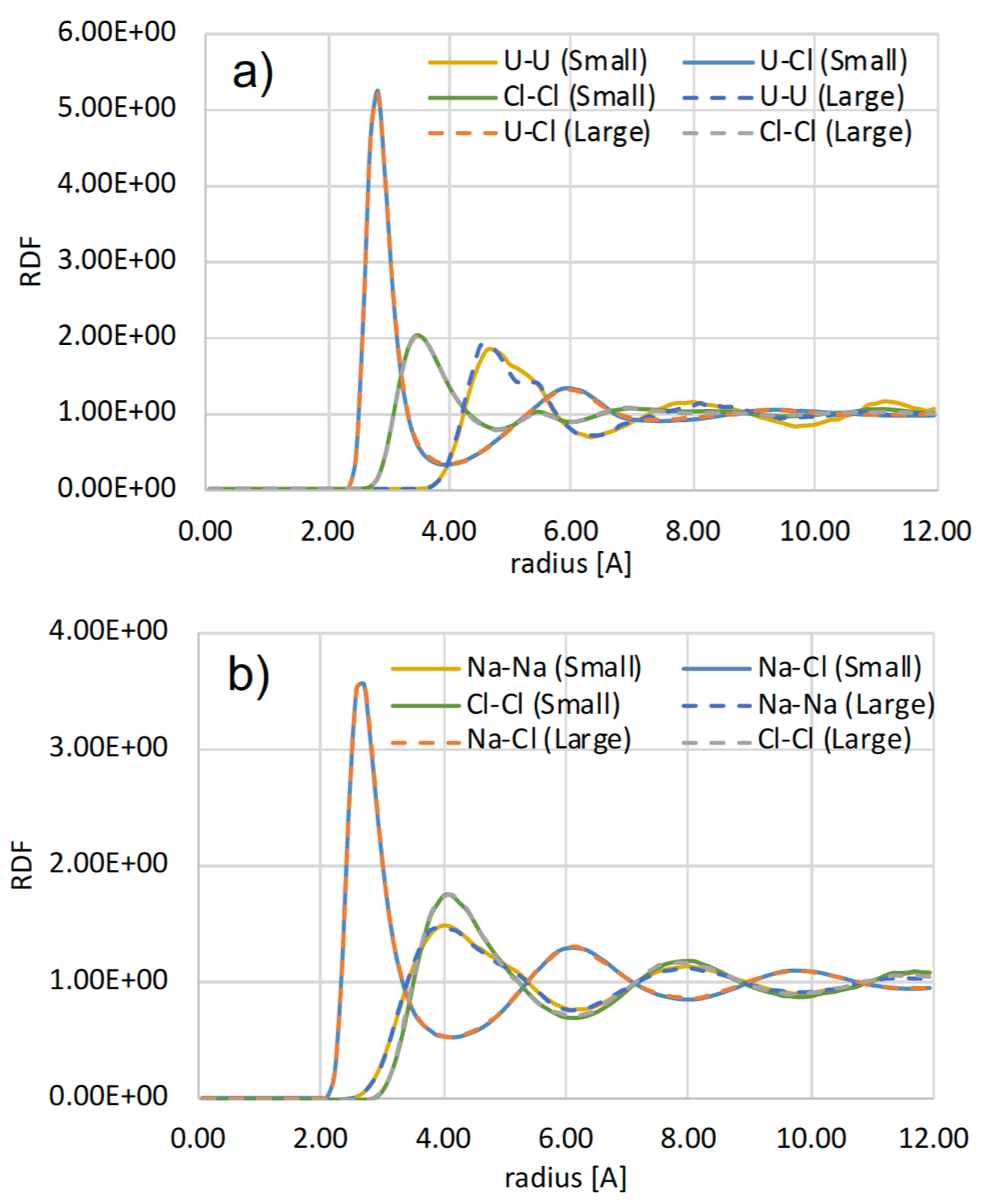
\includegraphics[width=0.45\textwidth]{./figures/FIG1_0_BB.png}
\caption{The predicted radial distribution function for select cases compared to literature data.} 
\label{fig:radial}
\end{figure}

\subsection{Pseudopotential and Van der Waals Dispersion}

The Projector Augmented Wave (PAW) method was used to describe the core electrons~\cite{}. For each element, the PAW potentials supplied with VASP for the PBE exchange-correlation potential were utilized. For Na, the version that only includes the s electron(s) in the valence shell was used for some of the simulations, while others use the version that also includes the semi-core p electrons. The difference between the two potentials will be discussed in Sec. \ref{sec:results}. Calculation of, for example, mixing energies in UCl$_3$-NaCl, can only be performed using a self-consistent data set (the same PAW potential), a rule which is carefully enforced in the present study. The PAW potential for Cl also included p electrons and for U it included the outer s, p and f electrons in the valance shell. 

It is well-established in the literature that Van der Waals or dispersion interactions are critical for reproducing the density of molten salts by DFT methods~\cite{}. Previous simulations have used both the DFT-D3 method~\cite{} and the Langreth \& Lundqvist~\cite{dion2004} methodologies for various molten chloride salts. Both methods are used in the present study and for the Langreth \& Lundqvist methodology the DF2 ~\cite{klime2009} exchange-correlation was tested. In addition, the so-called dDsC method was also included in the set of Van der Waals models \cite{}. The dDsC method does not include parameters for f elements in the standard VASP version. In order to enable simulations the corresponding parameters were taken from Ref. \cite{}. 



For some of the Van der Waals models, an alternate exchange-correlation potentials was utilized (rPW86~\cite{}). 

\subsection{Hubbard $U$ and Magnetism}

The generalized gradient approximation can fail to describe systems with localized (strongly correlated) f-electrons. This is often remedied by applying a Hubbard-like term to treat the strong on-site Coulomb interaction, commonly referred to as DFT+$U$ (also LDA+$U$ or GGA+$U$) \cite{rohrbach2003}. Calculations for U ions were performed with a Hubbard $U$ term, in order to capture the impact of accounting for strong electron correlation effects. 

Both the Dudarev and the Lichtenstein approach~\cite{dudarev1998} were used for the Hubbard $U$ methodology. As long as a self-consistent set of data is used, the choice of the Dudarev or Lichtenstein approaches does not materially influence the results. For the Lichtenstein approach, an approximate $U$ value range of 3.0-4.5 eV was determined by using scoping constrained DFT linear-response method for crystalline UCl$_3$~\cite{} while the $J$ value was set to 0.51 eV. These values are similar to those proposed for UO$_2$~\cite{}. After confirming that the values for UCl$_3$ were close to those for UO$_2$, the values for UO$_2$ were adopted in the present study. For the Dudarev approach, density, bandgap, and energy per molecule were analyzed as a function of U-J (U$_{eff}$) in increments of 1 eV for both UCl3 and NaCl-33UCl$_3$ at 1250 K, in the ferromagnetic (FM) and anti-ferromagnetic (AFM) states, and will be discussed further below. Uranium ions in its 3+ state have localized magnetic moments. Both ferro-magnetic and anti-ferromagnetic (AFM) orderings were investigated. In the context of molten salts, the AFM option is similar to a random distribution with a total magnetic moment in the supercell close to zero. 

The equilibrium density was determined by constructing pressure as a function of volume curves as a function of U$_{eff}$ at 1250 K for both the FM and AFM states. There is a general trend of decreasing density with increasing U$_{eff}$, and that the AFM state predicts a slightly higher density (lower volume) than the FM state. These equilibrium volumes are then utilized to determine the electronic density of states and the energy per molecule of their respective systems. The electronic density of states of AFM UCl$_3$ with a U$_{eff}$ of 0 and 4 eV is shown in Fig \ref{fig:DOS}. It can be seen that at a U$_{eff}$ of 0 eV UCl$_3$ exists electronically as a conductor. It is known that this molten salt exhibits insulating properties \cite{} with at least a minimal band gap. With the application of the Hubbard $U$ term, an insulating electronic structure is induced. The magnitude of the bandgap changes as a function of the magnitude of Ueff, with no bandgap below $U$=2 eV, and the bandgap progressively increasing up to approximately 2.3 eV for a U$_{eff}$ of 5 eV. The magnitude of the bandgap of UCl$_3$ has not been experimentally determined, removing the possibility of fitting the U$_{eff}$ to the experimental bandgap. 

By analyzing the energy per formula unit, it was found that the preferred magnetic state changes as a function of U$_{eff}$, with FM being preferred in the low U$_{eff}$/conducting region, and the AFM state preferred in the high U$_{eff}$/insulating region. It is theorized that at high temperatures one would not expect an ordered series of spins, and that is confirmed within this work, given that the electronic structure is appropriately accounted for. While a value of U$_{eff}$ greater than 2 eV is required to ensure the proper insulating electronic structure and magnetic state, the actual magnitude of the optimal U$_{eff}$ value remains unclear. Future work may consider further optimization of the Hubbard $U$ (and $J$) parameters, but the results and conclusions are not expected to significantly change based on this choice, as long as the value is sufficiently large to ensure an insulating ground state. For this work within the Dudarev approach, a U$_{eff}$ value of 4 eV was chosen, which corresponds with the choice of $U$ and $J$ from the Lichetenstein approach.

%It should be noted that the effective $U$ value depends on the coordination environment and consequently could differ between crystalline UCl$_3$ and molten salts.  It could also be a function of time in the simulations as the environment may change. Future work may consider these questions in more detail, but it is beyond the scope of the present study. The effect of the Hubbard $U$ parameter for molten uranium chloride salts is the same as for crystalline UO$_2$; without the $U$ parameter the salts are predicted to be metallic, which is contrary to the expected behavior, see Fig. \ref{fig:DOS}. Even though useful results may certainly be obtained while ignoring the strong correlations captured by the Hubbard $U$  model and accepting the resulting metallic character predicted for the salts, there are limitations to this approach. For reference, a few simulations were performed without the Hubbard $U$ model. 

%The AFM ordering is slightly energetically preferred and sometimes results in better convergence behavior. However, the predicted properties are not strongly influenced by the magnetic ordering.

%than PBE, such as XX, were used.
%For the uranium 5f electrons, an additional Hubbard $U$  term was introduced in order to capture the effect of strong correlations. 
%Calculations were also performed with the standard exchange-correlation potential (no Hubbard $U$ model). 

%Uranium ions in its 3+ state have localized magnetic moments. Both ferro-magnetic and anti-ferromagnetic (AFM) orderings were investigated. In the context of molten salts, the AFM option is similar to a random distribution with a total magnetic moment in the supercell close to zero. The AFM ordering is slightly energetically preferred and sometimes results in better convergence behavior. However, the predicted properties are not strongly influenced by the magnetic ordering. %Both the AFM and FM orderings are adopted in our simulations under the assumption that the thermodynamics and thermo-physical properties are only marginally affected by the choice. 
%Moreover, relative properties such as mixing energies or densities as function of temperature always use a self-consistent set of assumptions (the same magnetic ordering). 
%To end this discussion, we emphasize that even though the technical details differ between some data sets, results are only reported for self-consistent sets (using the same methodology for relative quantities) and any impact on the final results were evaluated to be within the range of general uncertainties before undertaking comparisons of properties derived from the different data sets. 

\begin{figure}[htb]
\centering
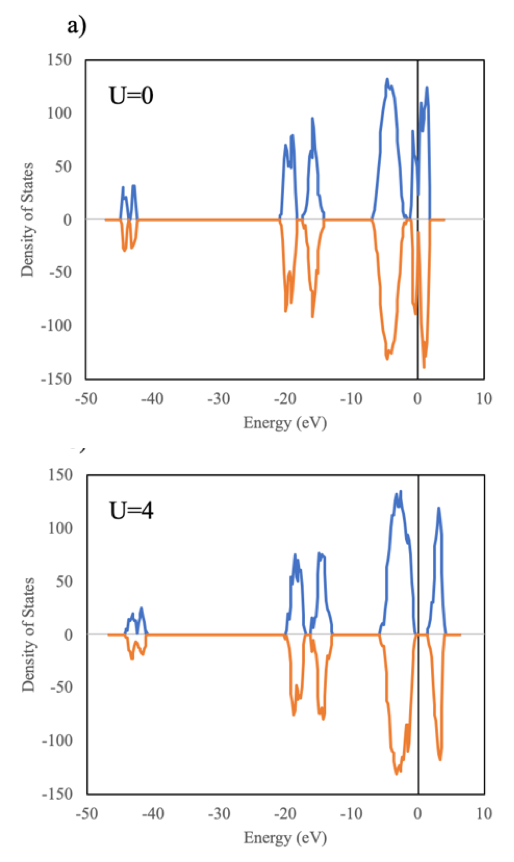
\includegraphics[width=0.45\textwidth]{./figures/figure2.png}
\caption{The predicted density of states for simulations of molten UCl$_3$ at 1250 K, a) including and b) not including a Hubbard $U$ model.} 
\label{fig:DOS}
\end{figure}


%The supercells of molten salts were either created by melting the crystalline phases at high temperature for an expanded volume using an isochoric (NVT) thermostat with velocities scaled each time step or by XXX. The temperature used for melting the lattice was well above the experimental melting point. The temperature of the system was then slowly reduced to the simulation temperature of interest. These simulations were performed with lower accuracy settings than the equilibration and production runs described above. The melting procedure was only performed once for a specific temperature in the middle of the range of interest. Simulations for other temperatures were performed by decreasing or increasing the temperature from the initial molten reference structure created according to the procedure above.

\subsection{AIMD simulations}
The AIMD simulations for the molten salt supercells were performed using both isobaric (NPT) and isochoric (NVT) conditions. The primary intent of the NPT simulations (with the pressure set to zero) is to evaluate density, thermal expansion, heat capacity and mixing energy. The NVT simulations also allow calculation of the compressibility and species diffusion. Both the NPT and NVT ensemble simulations applied the Langevin thermostat in VASP. For NVT simulations the equilibrium volume was determined by identifying the volume corresponding to zero pressure from a set of data points interpolated by an equation of state. 
The temperature friction coefficients were set to 10 ps$^{-1}$ and the friction coefficient for the lattice degrees of freedom (for NPT) to 1 ps$^{-1}$. The time step was set to 2 fs or lower for production runs between \~1000 K and 1500 K. Around and below 1000 K a larger time step, up to 5 fs, is warranted due to the slow dynamics of uranium ions. In principle, the larger time step can also be applied at higher temperatures as long as the structures have been properly converged. 
%, and 1 fs above this temperature. 

The simulations used pre-equilibrium runs that involve melting the lattice and ensuring convergence of the total energy and pair distribution function for the temperature of interest. After pre-equilibration, production runs follow for at least (about) 20 ps, of which the final 15 ps were used to calculate properties. The 20 ps were either reached by performing consecutive runs or by combining results for independent simulations over a shorter period of time. For example, five independent runs were performed for 5 ps of which the final 4 ps were used to calculate properties. This is assumed to yield approximately the same results as running a single simulation for 20 ps with the first 5 ps as preproduction time. Performing independent runs allow utilization of computational resources in a more efficient way. Some simulations used longer simulation times, in particular this applies to the simulations based on smaller supercells (up to 50 ps) and systems containing a mixture of UCl$_3$ and NaCl (up to 40 ps). NPT simulations often require long pre-equilibration runs. 

%None of the results change significantly after the minimum simulation time stated above (20 ps with a production time of 15 ps).
%Pre-equilibrium runs were performed with a time-step of 5 fs. The pre-equilibration runs were performed for a minimum of 10 ps. Production runs were performed for a minimum of 10 ps for all systems, higher for NaCl and for the small supercells. The first 1-2 ps in the production runs were ignored in order to ensure that the results for the new time step was allowed to equilibrate. Obviously, longer runs would further improve statistics and would certainly be desired, but the convergence of thermo-physical and thermodynamic quantities was monitored and deemed to be sufficient for the present purpose.  
%which is rather large but motivated by the heavy uranium ions moving very slowly and the need to accumulate sufficient statistics to evaluate properties. 
%This time step still allows resolution of the dynamics of Na and Cl ions. Production runs were preceded by equilibration for at least 5 ps with data collected during a minimum of 15 ps. 

%\subsection{Property calculations}
All properties were calculated by averaging over the production run (not including the equilibration or pre-production time). Densities were trivially obtained from the supercell volume and heat capacities from the slope of the total internal energy ($E$) as function of temperature. 
\begin{equation}
C=\frac{\partial E}{\partial T}
\end{equation}
For the NPT ensemble, this corresponds to heat capacity at constant pressure and for the NVT ensemble, heat capacity at constant volume. Mixing enthalpies/energies were calculated from the potential energy of the mixed salt with pure NaCl and UCl$_3$ at the same temperature as the reference. 
\begin{equation}
E_{mix}=E(U_xNa_yCl_{3x+y})-xE(UCl_3)-yE(NaCl).
\end{equation}
The compressibility is calculated as the negative of the inverse equilibrium volume multiplied by the derivative of the volume as a function of pressure. The diffusivities are calculated from the mean square displacements (MSD) through the Einstein relation.
\begin{equation}
MSD(t)=\sum_i^N (\mathbf{r^i(t)} - \mathbf{r^i(0)})^2 =6Dt,
\end{equation}
where $i$ denotes an ion, $N$ is the total number of ions, $\mathbf{r^i}$ is position vector, D is the diffusivity and t is time. According to kinetic theory, the diffusivity is expected to follow
\begin{equation}
D=\mu \,k_{\text{B}}T,
\end{equation}
where $\mu$ is the mobility, $k_B$ is the Boltzmann constant and T is temperature. The mobility is calculated from the temperature dependence of the diffusivity which may also be related to the viscosity and size of each species according to the Stokes-Einstein equation. However, that correlation was not attempted here.

\section{Results}
\label{sec:results}
\subsection{AIMD simulations for NaCl}
\subsubsection{Density, structure and compressibility}
Figure \ref{fig:NaCldensity} plots the predicted density of molten NaCl as function of temperature for the DFT-D3, dDsC and DF2 dispersion models as well as simulations without any dispersion interaction. 
%The results refer to the supercell size that we consider best converged for each methodology, see caption and below for further discussion. 
A correlation derived from experimental data is also shown~\cite{}. All simulations reproduce the temperature dependence of the density obtained from experiments. However, as expected, only the simulations that account for dispersion interactions are within 10\% of the experimental density correlation. The best agreement is obtained for the Langreth \& Lundqvist and dDsC dispersion models, which are within 5\% or less of the experimental correlation across an extended temperature range. The calculated (Langreth \& Lundqvist and dDsC) and experimental correlation for the density as function of temperature are listed in Table~\ref{table:densityetc}. The radial pair distribution function at 1250 K is reported as Supplementary Information, which highlights a first-shell coordination distance and number of XX \AA and YY, respectively.   

\begin{figure}[htb]
\centering
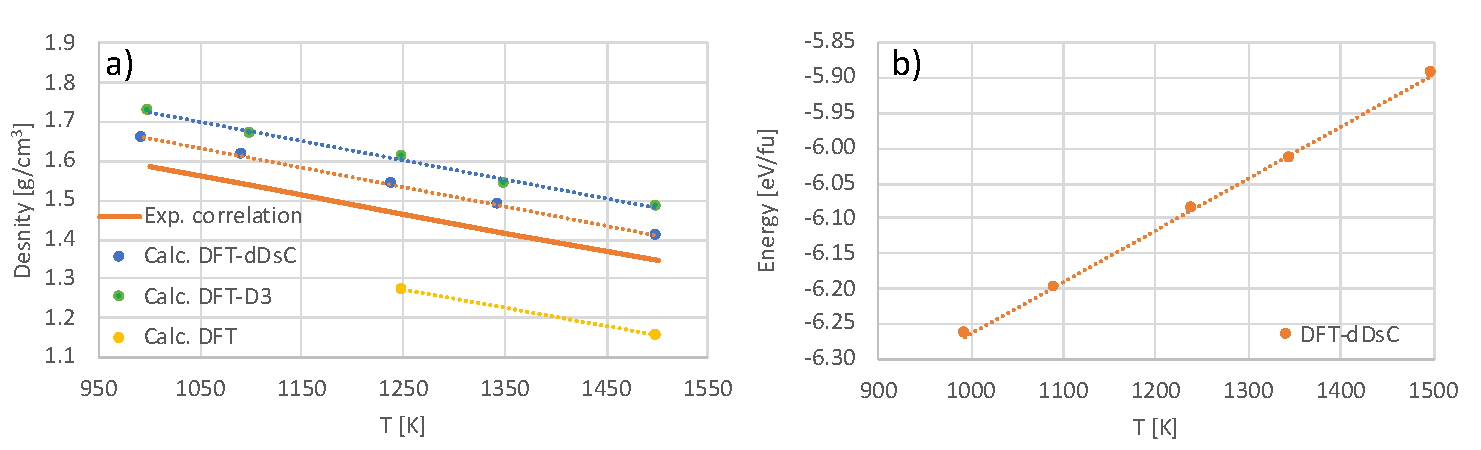
\includegraphics[width=0.45\textwidth]{./figures/FIG2.pdf}
\caption{Density of NaCl predicted with three different models for dispersion forces and one model without dispersion. Experimental data is represented by the correlation plotted as an orange line~\cite{}. %Note that the temperature range of the experimental correlation and some data points extend beyond the boiling point of NaCl, which is solely for illustrative purposes. 
The lines shown are linear least-squares fits to the calculated data points.} 
\label{fig:NaCldensity}
\end{figure}

\begin{table*}[hb!]
\centering
\begin{tabular}{lcccccc}
\hline
\hline
& Density (g/cm$^3$) & &Heat capacity (J/mol/K) & &Compressibility (GPa) &\\
&a &b &a &b &a &b \\
\hline
NaCl (D3)	& & & & & - & - \\
NaCl (dDsC)	& & & & & - & - \\
NaCl (DF2)	& & & & & & \\
NaCl Expt.	& & & & & & \\
UCl$_3$ (DF2) & & & & & & \\	
UCl$_3$ (dDsC) & & & & & - & - \\	
UCl$_3$ Expt.	& & & & & & \\
\hline
\hline
\end{tabular}
\caption{Calculated and experimental correlations for density, heat capacity and compressibility as function of temperature for NaCl and UCl$_3$. The first quantity is a linear function of temperature, while the latter two are constants.}
\label{table:NaCldensityetc}
\end{table*}

The NVT simulations also allow calculation of the compressibility. These results are also summarized in Table \ref{table:NaCldensityetc} (compressibility). % and Table \ref{table:NaCldiffusivityetc}.

\subsubsection{Heat capacity} 
Fig. \ref{fig:NaClheatc} plots the total energy per formula unit of molten NaCl as function of temperature. The derivative equals the heat capacity of NaCl, which is also tabulated in Table \ref{table:NaCldensityetc} together with an experimental reference value~\cite{}. The results refer to the supercell size that we consider best converged for each methodology, see caption and below for further discussion. The simulation results indicate a constant heat capacity. The good agreement between simulations and experiments for the heat capacity further emphasizes the accuracy of the AIMD simulations.  

\begin{figure}[htb]
\centering
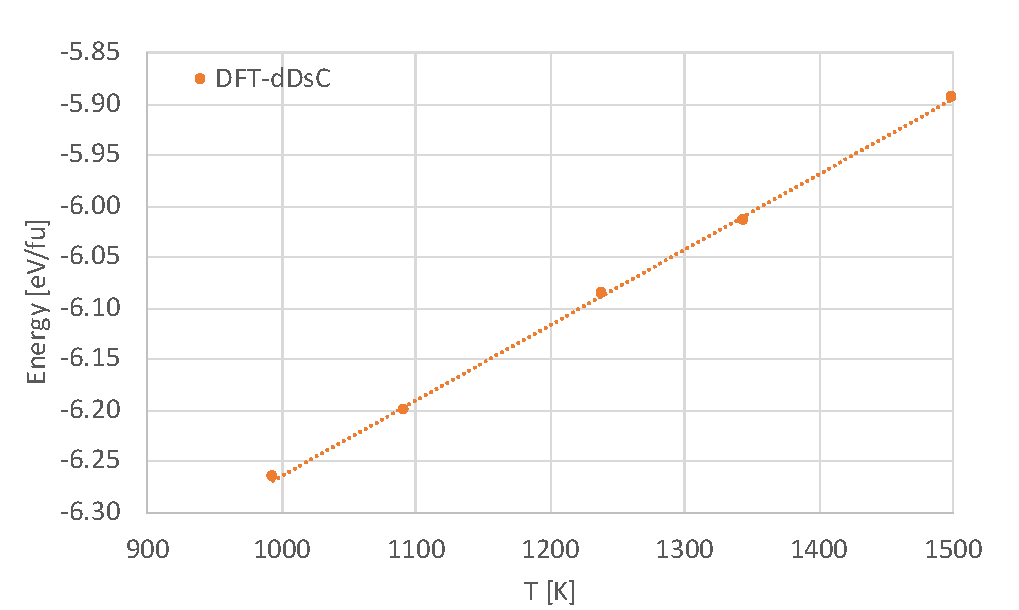
\includegraphics[width=0.45\textwidth]{./figures/FIG3.pdf}
\caption{Calculated total energy of NaCl as function of temperature. The line is a least-squares fit to data points and the slope represents the heat capacity.} 
\label{fig:NaClheatc}
\end{figure}

\subsubsection{Diffusivity} 
The AIMD simulations also allow calculation of the diffusivity of each species. These simulations work best in the NVT ensemble, consequently the results in Fig. \ref{fig:diffNaCl} only refer to simulations performed with that methodology. 
%These results are summarized in Fig. \ref{fig:diffNaCl}. 
As expected the diffusivity is a linear function of temperature in most of the temperature range, but with a clear tapering off as the meting point is approached. %, with a much stronger temperature dependence for Cl than for Na. 
The mobility of each species may be derived from the slope of the diffusivity as function of temperature (see Table \ref{table:NaCldiffusivityetc}). 


\begin{figure}[htb]
\centering
\includegraphics[width=0.45\textwidth]{./figures/FIGDiffNaCl.pdf}
\caption{Calculated diffusivities for each species in NaCl as function of temperature.} 
\label{fig:diffNaCl}
\end{figure}

\begin{table*}[hb!]
\centering
\begin{tabular}{lccc}
\hline
\hline
&Na	(m$^2$/s)&Cl (m$^2$/s)&U (m$^2$/s)\\
\hline
Mobility NaCl & & &\\
Mobility UCl$_3$	& & &\\
%Diffusivity NaCl-UCl$_3$ & & &\\
\hline
\hline
\end{tabular}
\caption{Calculated mobilites for each species in NaCl, UCl$_3$ and  NaCl-UCl$_3$.}
\label{table:NaCldiffusivityetc}
\end{table*}

\subsubsection{Impact of supercell size and other simulation settings}
The results in Figs. \ref{fig:NaCldensity} and \ref{fig:NaClheatc} refer to simulations based on the supercell that we consider best converged. Fig. \ref{fig:NaClsize} compares these results with those obtained from other supercells. Density and heat capacity are accurately represented by all supercell sizes in the temperature range investigated.
%smaller supercells, at least below 1750 K, which supports the accuracy of the results with respect to the supercell size. 
 These results suggest that for NaCl, the larger supercell is not required to achieve converged results for density and heat capacity at moderate temperature, which is consistent with the discussion of radial distribution functions in Sec. \ref{sec:method}. Consequently, the converged results in Figs. \ref{fig:NaCldensity} and \ref{fig:NaClheatc} as well as the correlations in Table \ref{sec:NaCldensityetc} are representative of all simulation results in this study, regardless of the supercell size. %Some deviation is observed for the highest temperature, which may be related to approaching the boiling temperature. 

\begin{figure}[htb]
\centering
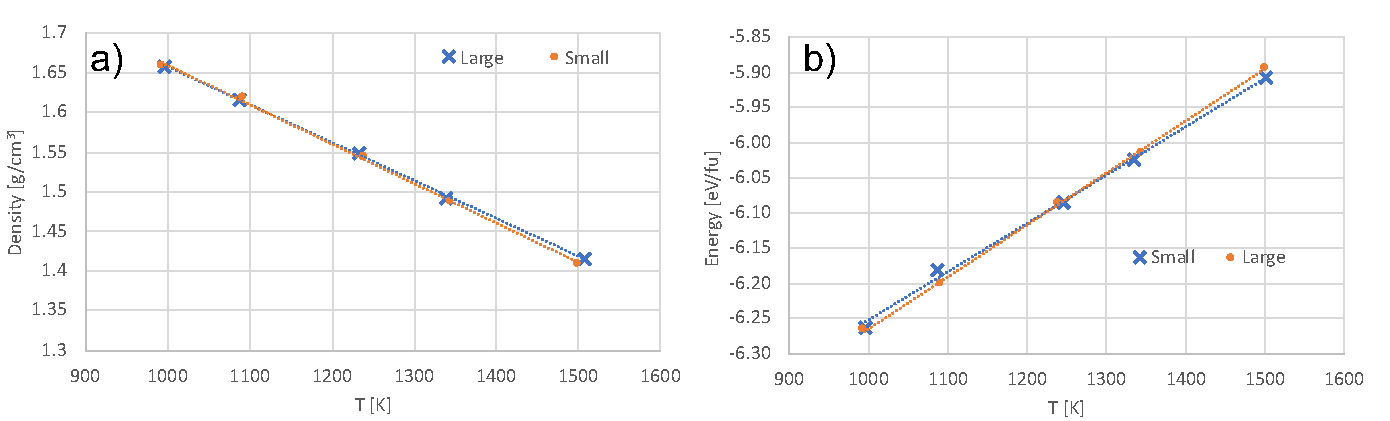
\includegraphics[width=0.45\textwidth]{./figures/FIG3b.pdf}
\caption{a) Calculated density and b) total energy of NaCl as function of temperature for the large and small supercells. The line is a least-squares fit to data points and the slope represents the heat capacity.} 
\label{fig:NaClsize}
\end{figure}

%The NVT simulations also allow calculation of the compressibility and diffusivity of each species. These results are also summarized in Table \ref{table:NaCldensityetc} (compressibility) and Table \ref{table:NaCldiffusivityetc}.

\subsection{AIMD simulations for UCl$_3$}
\subsubsection{Density, structure and compressibility}
Following the results for NaCl, the best performing Van der Waals models (Langreth \& Lundqvist and dDsC) were applied to UCl$_3$. % with a few spot checks using the other Van der Waals models as well. 
Figure \ref{fig:UCl3density}a) plots the predicted density for UCl$_3$ as function of temperature for the Langreth \& Lundquist and dDsC dispersion models. 
These results refer to the supercell size that we deem to be best converged and most representative of the UCl$_3$ system, see below for further discussion. 
The figure also compares the predicted densities to two (older) literature correlations derived from experiments~\cite{} as well as more recent experimental data points~\cite{}. 
%The inset highlights the difference in energy between the AFM, FM and non-magnetic simulations. 
%Figure \ref{fig:UCl3density}b) also includes results from simulations that do not include the Hubbard $U$ model for the U 5f electrons. 
The two (older) experimental correlations for density are surprisingly different and cannot both be correct, except in a narrow temperature range. The more recent experimental data~\cite{} confirm the model due to XX et al.~\cite{}, which are also consistent with the present AIMD simulations. Both the Langreth \& Lundqvist and dDsC models predict density values within a few per cent of these experimental data.
% The most recent experimental data set agrees well with the simulation data, with both the Langreth \& Lundqvist and dDsC model predicting values within a few per cent of the experimental data. 
 The temperature dependence is predicted to be close to linear across the full temperature range investigated. %The Langreth \& Lundqvist methodology is sensitive to the choice of exchange -correlation potential. The optimal choice proved excellent agreement with experiments, while other choices may lead to significant underestimation of the density despite performing very well for the NaCl benchmark system. 
 %Note that only a single point was calculated for the DFT-D3 model, but that indicates essentially the same behavior as the dDsC model.  
 Compared to the Desytniak correlation~\cite{}, the predicted temperature dependence of the density is slightly different. It agrees better with the more recent experimental data points~\cite{XX}. The densities in Figure \ref{fig:UCl3density} were fitted to linear correlations and summarized in Table \ref{table:NaCldensityetc}. 
 
The radial pair distribution function at 1250 K is reported as Supplementary Information, which highlights a first-shell coordination distance and number of XX \AA and YY, respectively. The coordination distance is in excellent agreement with the experimental values of 2.84 \AA~\cite{} and 2.85 \AA~\cite{} at 1200K, while it is higher than the AIMD simulations by XX et al., which can likely be ascribed to the application of the Hubbard $U$ methodology in the present study. The predicted coordination numbers are within the 6 to 8 range reported in previous experiments and simulations. %The U-U radial distribution function tends to zero slower than the 
 
Figure \ref{fig:UCl3density}b) compares the results in Fig. \ref{fig:UCl3density}a), which assume AFM (or random) ordering of magnetic moments, with results from simulations assuming FM ordering and simulations that do not include the Hubbard $U$ model for the U 5f electrons, both data sets were obtained for the Langreth \& Lundquist Van der Waals model. 
 The effect of including the Hubbard $U$ model is to decrease the density (increase the volume) compared to the reference case, which is consistent with the increase in volume observed for solid state simulations using the Hubbard $U$ methodology. The results without the Hubbard $U$ parameter is slightly closer to the densities measured in experiments. The magnetic order has a very small influence on the predicted density, which is highlighted in Figure \ref{fig:UCl3density}b). %We believe that the AFM (random) distribution is more representative of the high-temperature behavior of molten salts, as it should exhibit the lowest free energy (see below).

\begin{figure}[htb]
\centering
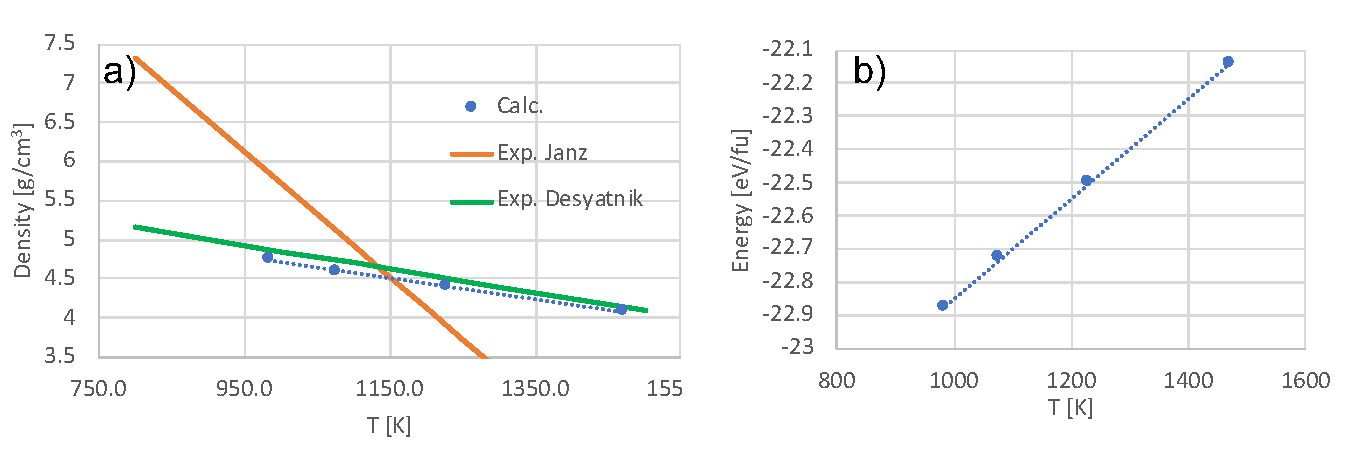
\includegraphics[width=0.45\textwidth]{./figures/FIG4.pdf}
\caption{a)Density of UCl$_3$ predicted with different models for the dispersion forces and one without. Experimental data is represented by the correlations plotted as blue lines and XX.~\cite{}. The lines are least-squares fits to the calculated data points, the equations of which are summarized in Table \ref{table:NaCldensityetc.} b)...} 
\label{fig:UCl3density}
\end{figure}

As for NaCl, The NVT simulations also allow calculation of compressibilty. These results are  summarized in Table \ref{table:NaCldensityetc} (compressibility). % and Table \ref{table:NaCldiffusivityetc}.

\subsubsection{Heat capacity} 
Figure \ref{fig:fig:UCl3heat} plots the total energy as function of temperature, from which the heat capacity can be derived by calculating the slope. The total energy closely follows a linear relation as function of temperature and, consequently, the heat capacity can be approximated as a constant in the temperature range investigated. 
We have not been able to identify experimental data on UCl$_3$, but our results compare very well with the value derived from the current CALPHAD UCl$_3$ database (see Table~\ref{table:NaCldiffusivityetc})~\cite{}. Figure \ref{fig:fig:UCl3heat}b compares the total energy as function of temperature for simulations assuming different magnetic ordering. The AFM (random) ordering is predicted to be slightly more stable than the FM ordering, though the difference is small. The AFM (random) model would be further stabilized by the magnetic entropy originating from the random distribution of magnetic moments at finite temperature. Consequently, the AFM (random) distribution of magnetic moments is considered to be the most representative model. %, which confirms AFM (random) ordering as the most appropriate model for production simulations. 

\begin{figure}[htb]
\centering
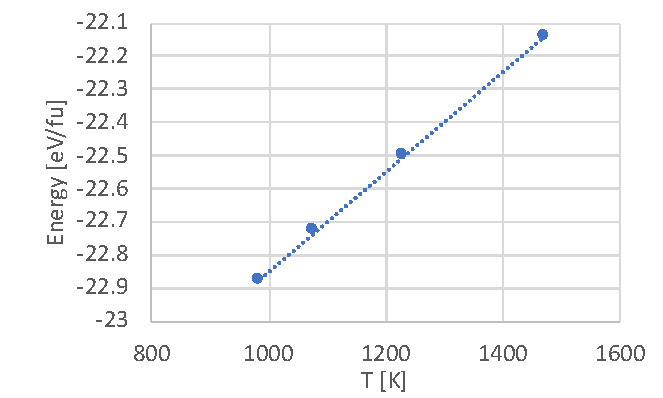
\includegraphics[width=0.45\textwidth]{./figures/FIG5.pdf}
\caption{Calculated total energy of UCl$_3$ as function of temperature. The line is a least-squares fit to data points and the slope represents the heat capacity.} 
\label{fig:UCl3heat}
\end{figure}

\subsubsection{Diffusivity}
As for NaCl, The AIMD simulations also allow calculation of the diffusivity of each species. Again similar to the NaCl system, these simulations work best in the NVT ensemble and results are only report for that case, see Fig. \ref{fig:diffUCl}. As expected, the diffusivity is a linear function of temperature. %, with a much stronger temperature dependence for Cl than for U. 
The mobility of each species may be derived from the slope of the diffusivity as function of temperature (see Table \ref{table:NaCldiffusivityetc}). 

\begin{figure}[htb]
\centering
\includegraphics[width=0.45\textwidth]{./figures/FIGDiffUCl.pdf}
\caption{Calculated diffusivities for each species in NaCl as function of temperature.} 
\label{fig:diffNaCl}
\end{figure}

\subsubsection{Impact of supercell size and other simulation settings}
The results discussed above for UCl$_3$ refer to simulations using the supercell size that we deem to be best converged and most representative of the UCl$_3$ system for each simulation methodology. Select results obtained from different supercell sizes are compared in Fig. \ref{fig:UCl3size}, which, similar to NaCl, exhibits good agreement with each other.  Any difference between supercell sizes is primarily ascribed to sampling appropriate configurations rather than an effect of increasing the numbers of ions in the simulation box, although additional simulations would be required to fully certify this conclusion. 

\begin{figure}[htb]
\centering
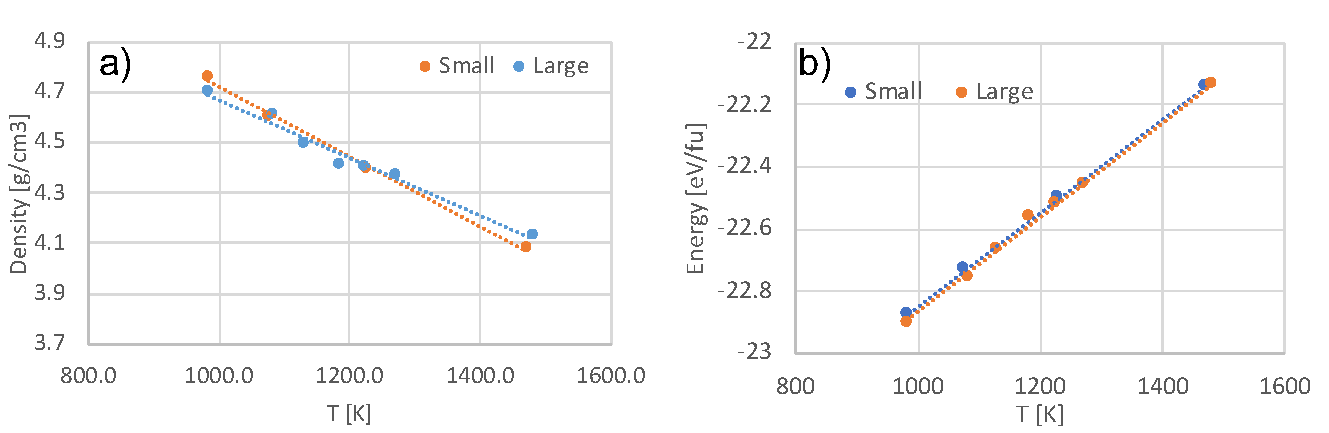
\includegraphics[width=0.45\textwidth]{./figures/FIG4b.pdf}
\caption{Calculated density and total energy of UCl$_3$ as function of temperature for the large and small supercells. The line is a least-squares fit to data points and the slope represents the heat capacity.} 
\label{fig:UCl3size}
\end{figure}

%As for NaCl, The NVT simulations also allow calculation of the compressibility and diffusivity of each species. These results are  summarized in Table \ref{table:NaCldensityetc} (compressibility) and Table \ref{table:NaCldiffusivityetc}.
 
\subsection{AIMD simulations for NaCl-UCl$_3$}
\subsubsection{Density, structure and compressibility}
The density of NaCl-UCl$_3$ mixtures were calculated for the Langreth \& Lundqvist and dDsC dispersion models at three or four (depending on composition) different temperatures between 800 K and 1500 K, as shown in Figure \ref{fig:NaClUCl3}a). This figure also includes densities at the same temperatures obtained from correlations derived from experimental data due to Desyatnik et al.~\cite{} and lines corresponding to an ideal mixture of the end members. Figure \ref{fig:NaClUCl3}b) highlights the fractional deviation from ideal solution behavior. 
It is challenging to converge the density for mixed salt solutions to an accuracy better than around a per cent of the absolute density using AIMD simulations, which give rise to some scatter in the data points. Nevertheless, a few trends are discernible from Figure \ref{fig:NaClUCl3}. The simulation data points are within a few per cent of the experimental data and close to the ideal mixture. The dDsC simulations within the NPT ensemble suggest a negative deviation from an ideal solution (lower density than predicted by an ideal solution behavior) by up to 2-3\%, except close to pure UCl$_3$. The magnitude of the deviation from ideal solution behavior is a function of composition and varies some with temperature in the UCl$_3$ rich part, while it is almost constant in the NaCl rich part according to the simulations. 
The maximum deviation from ideal solution behavior occurs close to the eutectic composition of 30\% UCl$_3$. These predictions are qualitatively similar to the correlations derived form experiments by Desyatnik et al.~\cite{}, though the experiments predict a larger magnitude for the deviation from an ideal solution and also exhibits a stronger temperature dependence than the simulations. The Langreth \& Lundqvist simulations within the NVT ensemble predict a close to ideal solution behavior across the full temperature and composition range.
  %  and experiments suggest a negative deviation from an ideal solution (lower density than predicted by an ideal solution behavior), except close to pure UCl$_3$ where experiments and simulations at T=1500K exhibit a positive deviation. Although experiments report the magntiude of the deviation from ideal solution to be a function of temperature, the highest deviation occurs at low temperatures, simulations predict a close to temperature independent deviation from ideal solution behavior. Both experiments and simulations predict a minimum in the deviation rom ideal solution close to the eutectic composition of 30\%, however simulations predict the magnitude of the deviation to be much smaller than experiments. 
%It is challenging to converge the density for mixed salt solutions using AIMD simulations, which give rise to some of the 
% . Although there is some spread in the data points that we ascribe to sampling uncertainties, there is a minimum about 3\% below the ideal solution density close to the eutectic composition. The experimental data also shows a negative deviation, including a minumum close to the eutectic composition.  

Figure \ref{fig:NaClUCl3_t}a) plots the density as function of temperature for each composition, which emphasizes a close to linear temperature dependence similar to the pure end-members. The corresponding linear equations for each composition are listed in Table \ref{table:density_data}. 
The coefficients describing the linear dependence on composition are plotted in \ref{fig:NaClUCl3_t}b). Although there is some scatter, there seems to be a weak quadratic dependence on composition for both the linear and constant term, except for $x_{UCl_3}=0.875$, which deviates slightly from the general trend for both parameters. The weak quadratic dependencies can be parametrized and used to express the temperature and composition dependent densities according to:
\begin{equation}
\end{equation}
These density correlations can be used for calculating densities at temperatures not explicitly investigated by AIMD simulations. % according to the following equations,
This approach is utilized to compare the AIMD predictions to the recent experimental data from Scott et al.~\cite{} in Fig. \ref{fig:NaClUCl3_comp} collected at XX and YY K. These experiments suggest that the density behaves much closer to an ideal solution than those due to Desyatnik et al.~\cite{}. The agreement with the AIMD predictions is still very good, considering uncertainties associated with both experiments and simulations.  

\begin{figure}[htb]
\centering
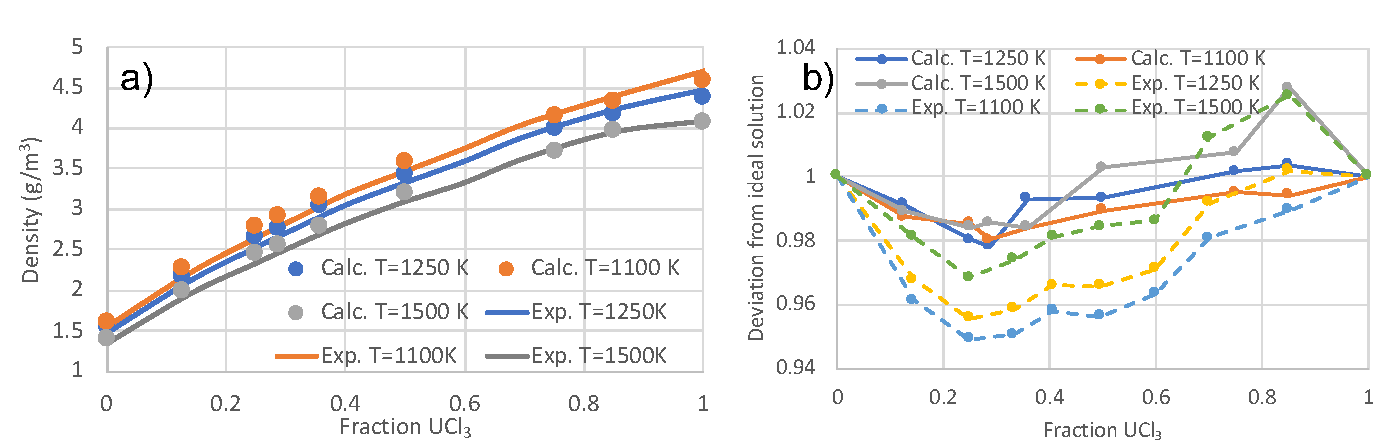
\includegraphics[width=0.45\textwidth]{./figures/FIG6.pdf}
\caption{a) Density of NaCl-UCl$_3$ mixtures as obtained from simulations and experimental data~\cite{} at temperatures between 800 K and 1500 K. The lines represent an ideal solution with the calculated and experimental NaCl and UCl$_3$ densities as end points. b) The deviation form ideal solution behavior is plotted as function of composition at temperatures between 800 K and 1500 K. %Results for both the large and small supercells are shown.
} 
\label{fig:NaClUCl3}
\end{figure}

\begin{figure}[htb]
\centering
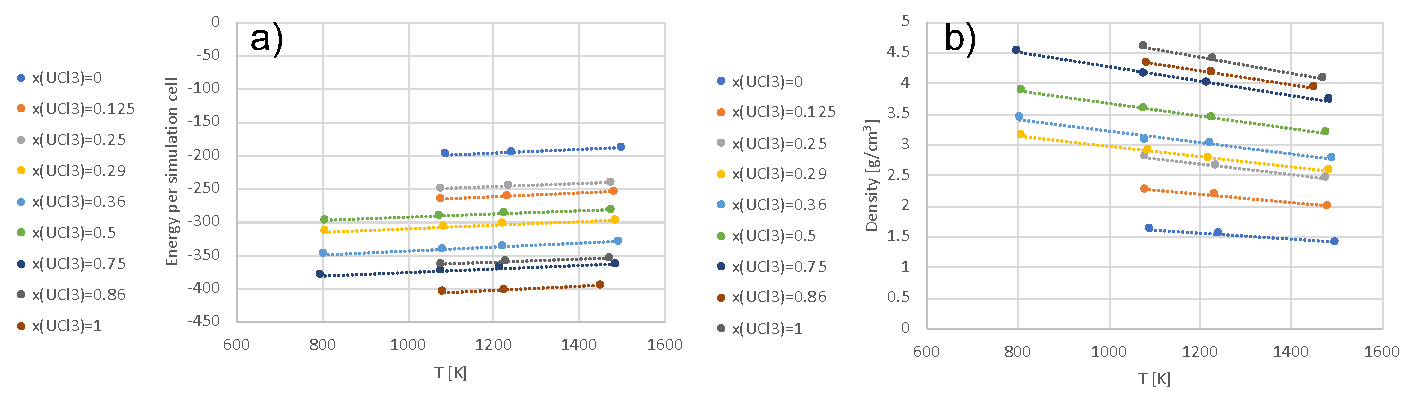
\includegraphics[width=0.45\textwidth]{./figures/FIG6c.pdf}
\caption{a)}. b). 
\label{fig:NaClUCl3_t}
\end{figure}

\begin{figure}[htb]
\centering
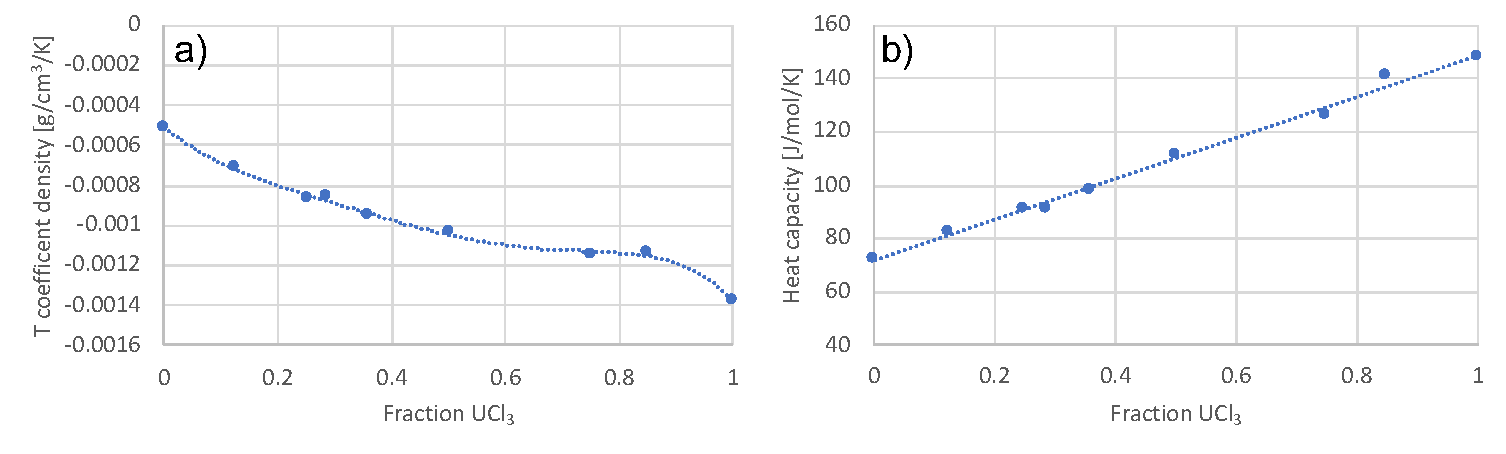
\includegraphics[width=0.45\textwidth]{./figures/FIG6f.pdf}
\caption{a)}. b). 
\label{fig:NaClUCl3_comp}
\end{figure}

\subsubsection{Mixing energy and heat capacity}
The potential energies of the NaCl-UCl$_3$ mixtures at temperatures ranging from 800 K to 1500 K are plotted in Figure \ref{fig:NaClUCl3e}a, with the NaCl and UCl$_3$ end members as reference points. The mixtures exhibit a negative deviation from ideal solution behavior, which implies that the solution phase is favored over a two-phase mixture of the end-points. Addition of entropy further stabilizes the mixed solution phase, as shown in Fig. \ref{fig:NaClUCl3e}b by adding a simple ideal solution model to the potential energy in Fig. \ref{fig:NaClUCl3e}b).
 The minimum (most negative) mixing energy is between the $x_{UCl_3$}=0.375 and  $x_{UCl_3$}=0.5, which qualitatively mimics the results for the density. The potential energy minimum may be shifted slightly closer to the 50-50 composition. However, it may be questionable if the simulations are sufficiently converged to draw such a subtle conclusion.  The Langreth \& Lundqvist and dDsC simulations predict very similar solution energies. The minimum of the free energy is shifted close to the 50-50 composition. 
 
 The solution energy was measured at 1100 K by XX et al. The results are shown in \ref{fig:NaClUCl3e}a) and indicate very good agreement with the simulations across the full temperature range. In addition to the experimental data points, there are two sets of thermodynamic models for the solution energy~\cite{}, see Figure \ref{fig:NaClUCl3e}a). Both thermodynamic models assume the solution energy to be independent of temperature, which is in good agreement with the simulations. The model by XX \textit{et al.} was derived from the experimental measurements and consequently agree well with our simulation results. The model by XX \textit{et al.} shows a smaller mixing energy than both experiential data points and simulations. 

%Although the simulations were run long enough to sample the configuration space, it is possible that the initial distribution of Na and U ions have some impact on the results, especially for the large supercells.  In order to test this possibility, a few of the Na And Cl atoms in the previous simulations were swapped and the simulations were re-run. In particular we target the compositions that seemed to deviate from the overall trend somewhat. Indeed, the new simulations provided slightly different results in closer agreement with the trends already discussed. For the large cells, this is an inherent uncertainty of the simulation apporach.

\begin{figure}[htb]
\centering
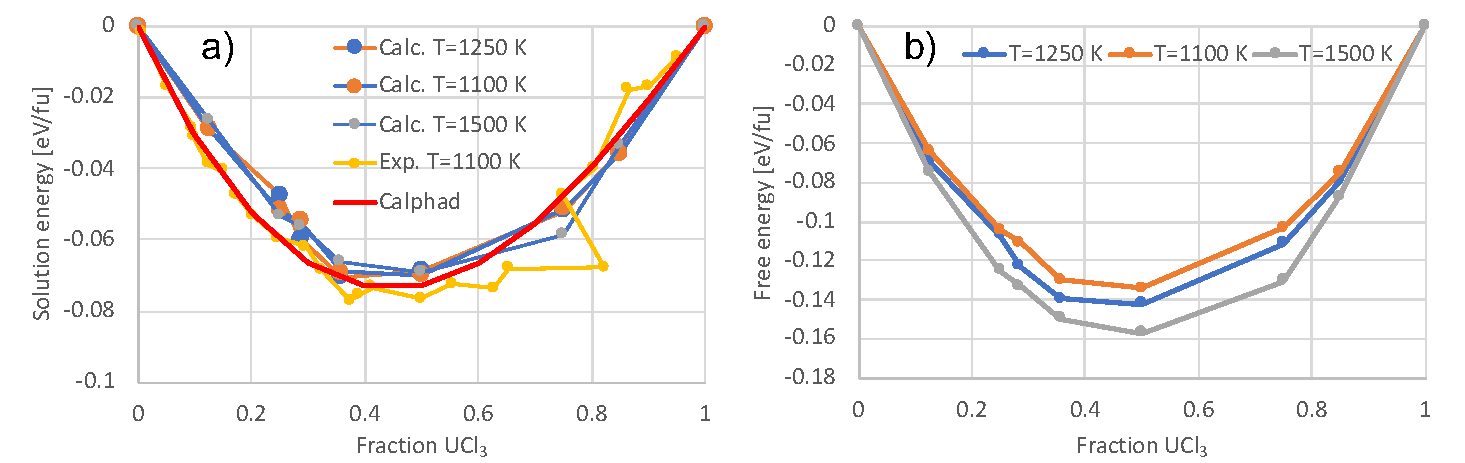
\includegraphics[width=0.45\textwidth]{./figures/FIG7.pdf}
\caption{a) Mixing energies for NaCl-UCl$_3$ mixtures at 1100 1250 and 1500 K. Pure NaCl and UCl$_3$ are used as references. The solid black line represents the zero-mixing energy for the ideal solution. %b) Same as a) but performed using a different simulation methodology at 1200 K. 
Results are shown for the best converged supercells. b) The free energy of mixing at 1100 1250 and 1500 K.} 
\label{fig:NaClUCl3e}
\end{figure}

The total energy for each UCl$_3$-NaCl composition is plotted as function of temperature in Figure \ref{fig:NaClUCl3t}a, from which heat capacity can be calculated as the slope, similar to the pure NaCl and UCl$_3$ systems. From Figure \ref{fig:NaClUCl3t}b, the heat capacity is a linear function of the salt composition, which is expected based on the lack of temperature dependence fo the salt mixing energies. The negative deviation from an ideal solution seen for the mixing energy and density cannot be distinguished for the heat capacity. 

Based on the results for the mixing energy and heat capacity, the following expression may be derived for the mixing energy as function of the composition and temperature:
\begin{equation}
\end{equation}

%The comparison between large and small supercells for the density and mixing energy are also shown in Figs. \ref{fig:NaClUCl3} and \ref{fig:NaClUCl3e}. Unlike the cases of NaCl and UCl$_3$, the NaCl-UCl$_3$ mixture exhibit some deviation between the supercells for one of the compositions, although the trends are still the same. 

\section{Discussion}
\label{sec:discussion}
The discussion section will focus on the behavior of mixed salts, in particular how the mixing properties (energy and density) relate to the evolution of the pair distribution functions in the mixed salts. Figure \ref{fig:fig_pair} plots the pair distribution functions at each salt composition and compares them to the reference pair distribution functions for NaCl and UCl$_3$ salts. 
Ref. \cite{} already showed that as NaCl is added to pure UCl$_3$, the number of Cl ions in the first neighbor shell around U ions increases, from 6 in UCl$_3$ to almost 8 close to NaCl, with a corresponding decrease around Na ions. This is also confirmed in the present study (see Figure \ref{fig:fig_pair}). This redistribution of Cl ions clearly represents a favorable interaction as the mixing energy is negative across the full composition range. The same study also identified networks of UCl$_3$ units above a fractional UCl$_3$ concentration of 0.30, and more isolated units below this concentration. This behavior is also visible in the pair distribution functions. The U-U pair distribution function for mixtures with a composition above a fractional UCl$_3$ concentration of 0.30 maintain the same shape and height as in pure UCl$_3$ (they essentially overlap), which emphasizes the importance of network formation in the mixtures. Below a fractional concentration of 0.30 the U-U pair distribution function rapidly deviates from the pure UCl$_3$, indicating an inability to maintain the favorable network structure. 
Related changes may be observed in other distribution functions. 
The location of this transition coincides with the minimum in the mixing energy and the maximum deviation of the density from an ideal solution (compare Figures \ref{fig:fig_pair},  \ref{fig:fig:NaClUCl3e} and \ref{fig:NaClUCl3)}. In turn, these coincide with the position of the eutectic composition according to the experimental phase diagram. Combined with the evolution of the U-Cl and U-U pair distribution functions in the mixtures, this suggest that the negative mixing energy is driven by increases in the Cl coordination around U ions, but if the fractional UCl$_3$ concentration is below 0.3, the gain from increasing this U-Cl coordination is countered by not being able to maintain the favorable U-U coordination seen in UCl$_3$, as evidenced by the break-up of the network structures. The balance of the increase in the U-Cl coordination and decrease in U-U coordination as function of the composition of UCl$_3$-NaCl salts is responsible for the minimum in the mixing energy and by extension the location of the eutectic point in the phase diagram. 

The negative deviation from an ideal solution exhibited by the density implies that the volume increases. Often, a negative mixing energy is associated with a stronger bonding and lower volume, clearly that is opposite to what is observed for NaCl-UCl$_3$. The reason for increased volume and decreased density is again related to the evolution of the pair distribution function. The increased coordination number of Cl around U ions means that the bonding environment starts to resemble that of U$^{4+}$ ions in UCl$_4$, which may also be what drives the favorable interaction. The density of UCl$_4$ is noticeably lower (and the molar volume higher) that that of UCl$_3$, which we believe correlates with the negative deviation form an ideal mixture for the density of UCl$_3$-NaCl. Note that analogy does not imply the presence of formal U$^4+$ ions in UCl$_3$-NaCl, but a partial transition that drives the evolution of both the mixing energy and density. Additional simulations and experiments would be required to provie this hypothesis.

 \begin{figure}[htb]
\centering
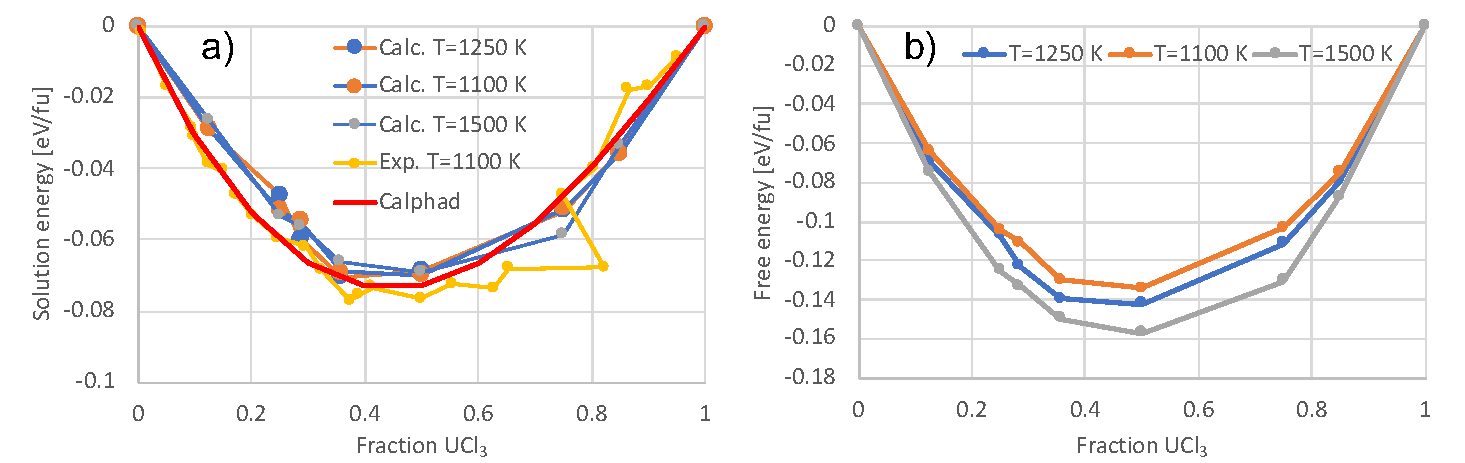
\includegraphics[width=0.45\textwidth]{./figures/FIG7.pdf}
\caption{Pair distribution functions for UCl$_3$-NaCl mixtures as function of composition. The reference U-Cl and U-U pair distribution functions for UCl$_3$ are plotted in each figure.} 
\label{fig:fig_pair}
\end{figure}



\section{Conclusions}
\label{sec:conclusions}


\section{Acknowledgments}



\bibliographystyle{elsarticle-num-names}
\bibliography{salt}

\end{document}
